\documentclass{fkssolpub}

\usepackage[czech]{babel}
\usepackage{fontspec}
\usepackage{fkssugar}
\usepackage{amsmath}
\usepackage{graphicx}

\author{Ondřej Sedláček}
\school{Gymnázium Oty Pavla} 
\series{3p}
\problem{1} 

\begin{document}

\begin{figure}[h!]
	\centering
	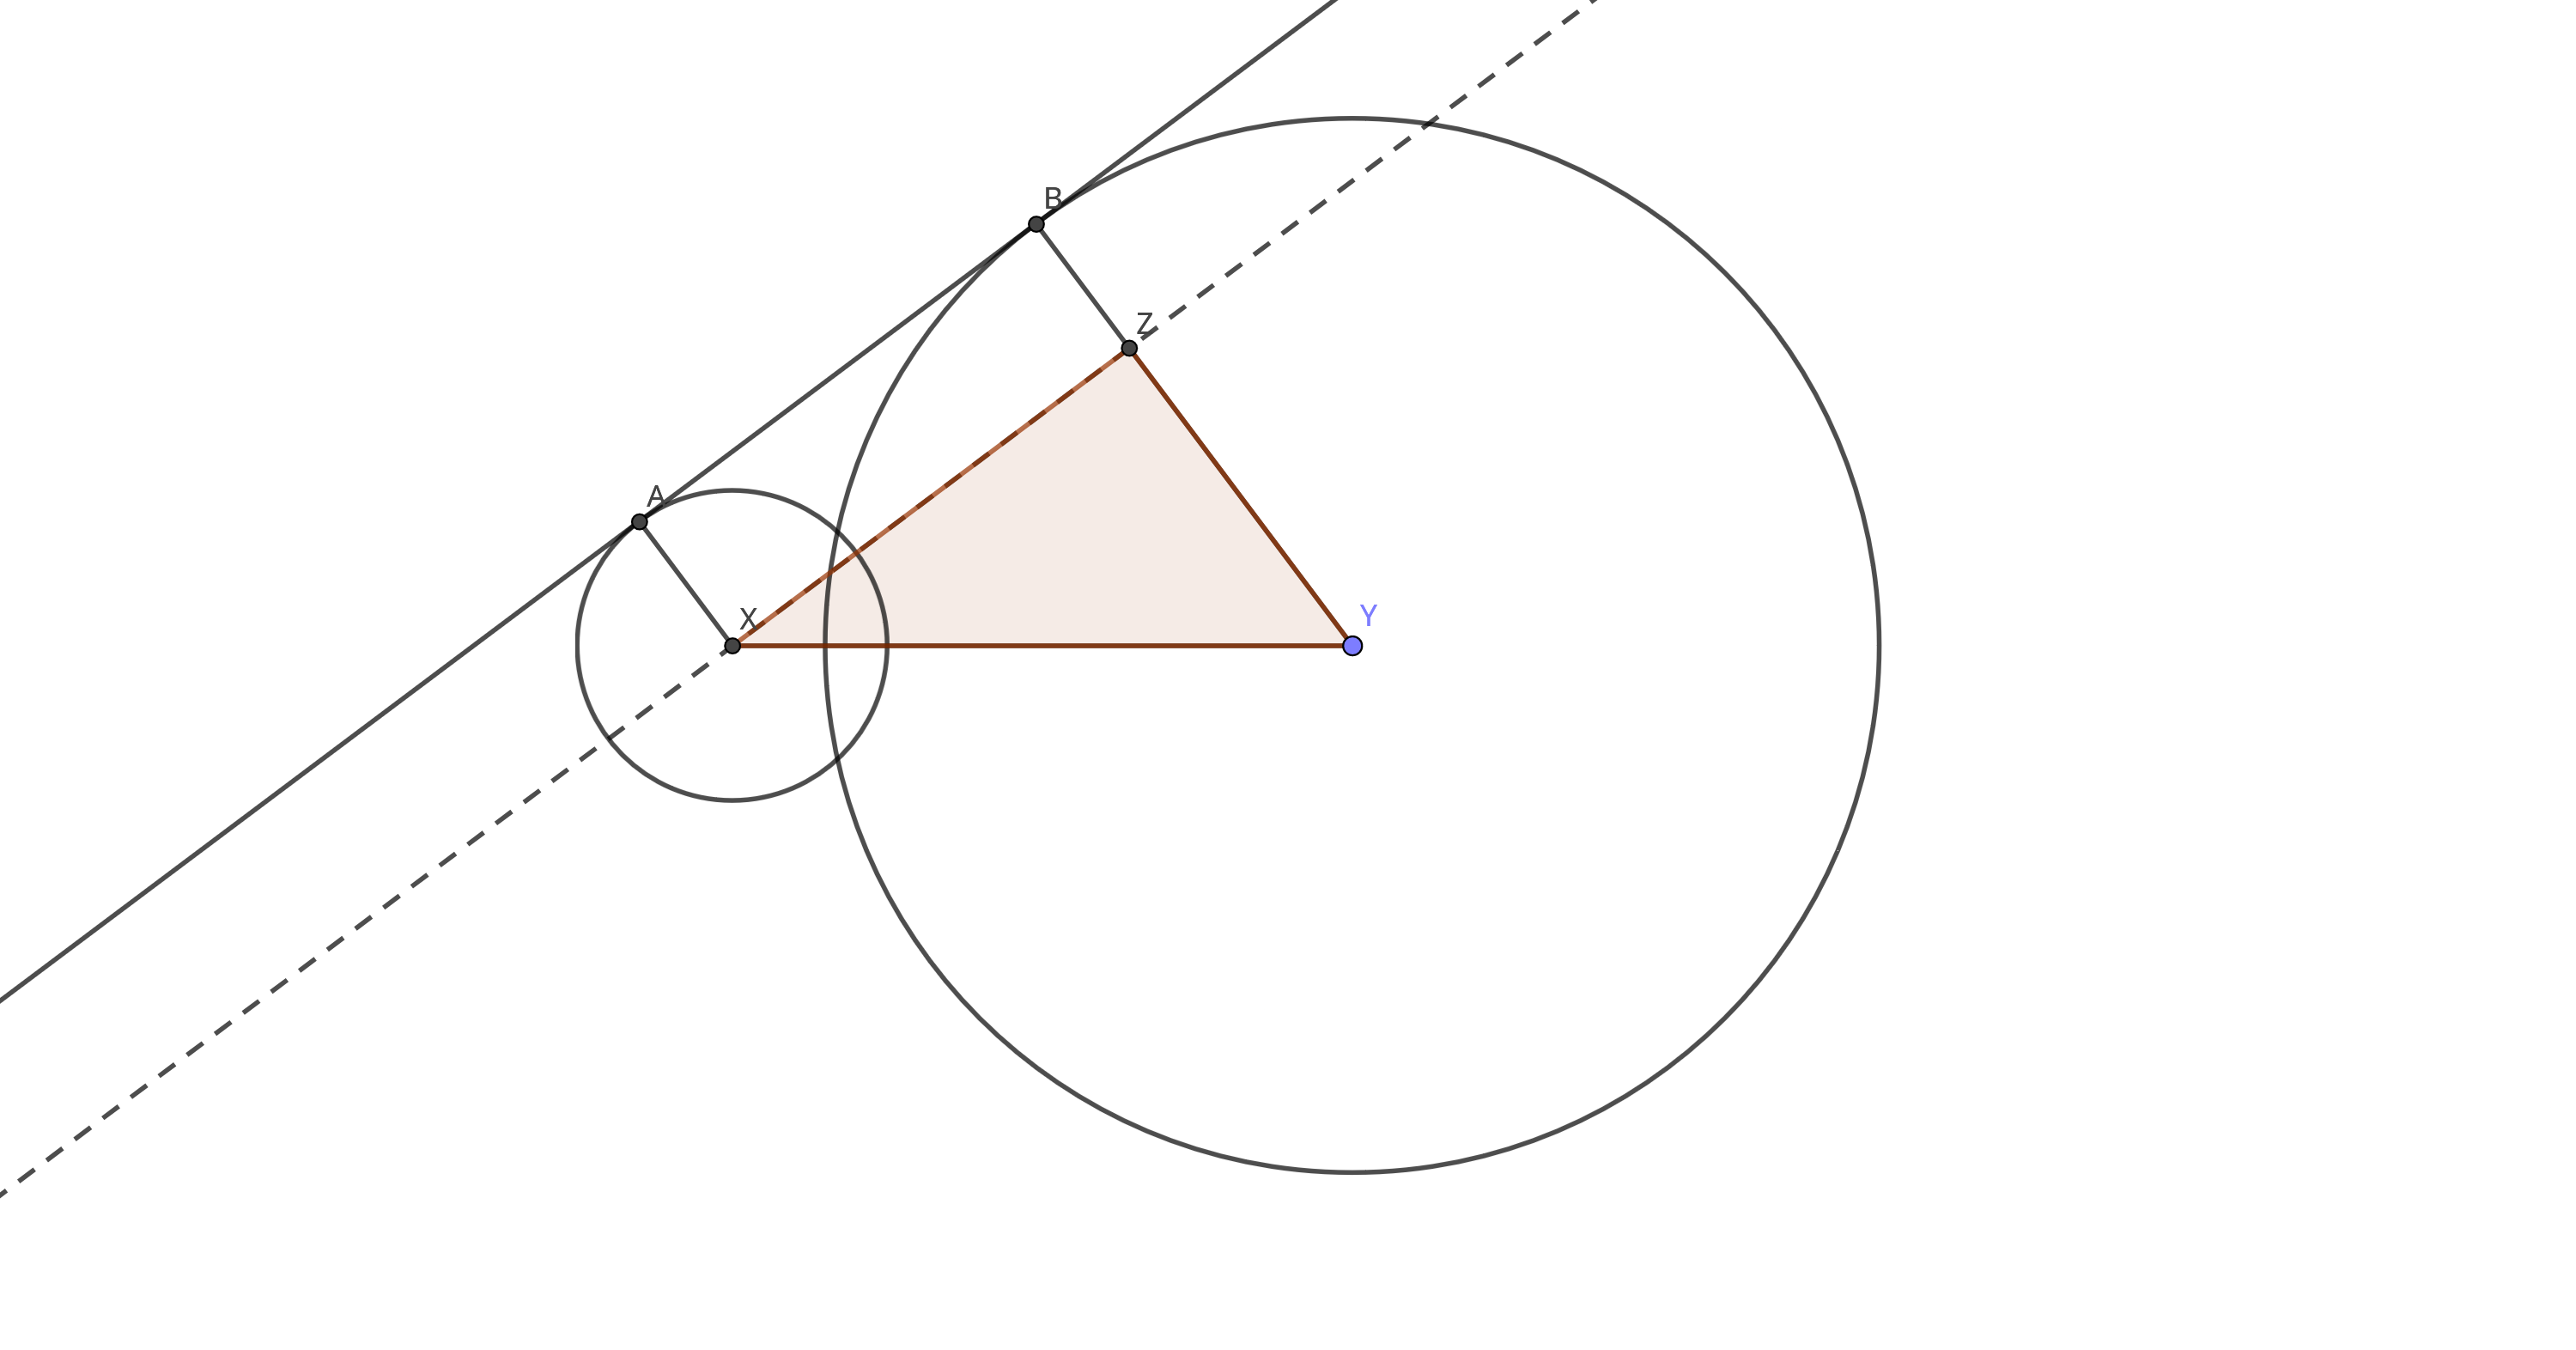
\includegraphics[width=\textwidth]{1-fig.png}
	\caption{Konstrukce ze zadání}
\end{figure}

Nechť střed první kružnice jsou $X$ a druhé $Y$. Teď zkonstruujeme rovnoběžku
s $AB$ procházející bodem $X$. Pak nechť průsečík této rovnoběžky se spojnicí
středu $Y$ a dotykového bodu $YB$ je $Z$. Protože $XA$ a $YB$ jsou spojnice
středu s dotykovým bodem,
je čtyřúhelník $ABZX$ obdélník proto velikost $|YZ| = |YB| - |XA|
	= 17 - 5 = 12$,. A protože $AB \perp YB$, pak taky $XZ \perp YZ$. Díky
tomu je tedy trojúhelník $XYZ$ pravoúhlý s pravým úhlem u $Z$, a protože
$|AB| = |XZ|$, dopočítáme $|XZ|$ přes Pythagorovu větu:

\[
	|YZ|^2 + |XZ|^2 = |XY|^2
\]
\[
	|XZ| = \sqrt{|XY|^2 - |YZ|^2}
\]
\[
	|AB| = |XZ| = 16
\]

Vyšlo nám, že $|AB| = 16$.


\end{document}
